\documentclass{beamer}
\usepackage[utf8]{inputenc}
\usepackage[T1]{fontenc}
%\usepackage[french]{babel}

\usepackage{amsmath}
\usepackage{amssymb}
\usepackage{color}
\usepackage{graphicx}

\usepackage{listings}
\lstset{ %
  backgroundcolor=\color{white},   % choose the background color; you must add \usepackage{color} or \usepackage{xcolor}
  basicstyle=\tiny,        % the size of the fonts that are used for the code
  breakatwhitespace=false,         % sets if automatic breaks should only happen at whitespace
  breaklines=true,                 % sets automatic line breaking
  captionpos=b,                    % sets the caption-position to bottom
  commentstyle=\color{green},      % comment style
  deletekeywords={...},            % if you want to delete keywords from the given language
  escapeinside={\%*}{*)},          % if you want to add LaTeX within your code
  extendedchars=true,              % lets you use non-ASCII characters; for 8-bits encodings only, does not work with UTF-8
  frame=single,                    % adds a frame around the code
  keepspaces=true,                 % keeps spaces in text, useful for keeping indentation of code (possibly needs columns=flexible)
  keywordstyle=\color{blue},       % keyword style
  language=xml,                    % the language of the code
  morekeywords={Level,Cache,Architecture,...},            % if you want to add more keywords to the set
  numbers=left,                    % where to put the line-numbers; possible values are (none, left, right)
  numbersep=5pt,                   % how far the line-numbers are from the code
  numberstyle=\tiny\color{blue},  % the style that is used for the line-numbers
  rulecolor=\color{black},         % if not set, the frame-color may be changed on line-breaks within not-black text (e.g. comments (green here))
  showspaces=false,                % show spaces everywhere adding particular underscores; it overrides 'showstringspaces'
  showstringspaces=false,          % underline spaces within strings only
  showtabs=false,                  % show tabs within strings adding particular underscores
  stepnumber=2,                    % the step between two line-numbers. If it's 1, each line will be numbered
  stringstyle=\color{red},         % string literal style
  tabsize=2,                       % sets default tabsize to 2 spaces
  title=\lstname                   % show the filename of files included with \lstinputlisting; also try caption instead of title
}

\usetheme{CambridgeUS}
\title[PFA - Simulateur de caches multi-c\oe ur]{PFA - Simulateur de caches multi-c\oe ur}
\author[]{Nicolas Dubois, Pierre Goudet, Nicolas Heng,\\Alexandre Honorat, Gilles Marait, Grégoire Pichon}
\institute[ENSEIRB-MATMECA]{ENSEIRB-MATMECA}
\date{\today}
%\date{}

\setbeamercolor{title}{bg=red!65!black,fg=white}

\begin{document}

\setlength{\unitlength}{1cm}

\begin{frame}{Présentation}

\titlepage

\end{frame}

%\AtBeginSection[]
%{
%\begin{frame}<beamer>
%  \frametitle{Plan}
%  \tableofcontents[currentsection]
%\end{frame}
%}

\begin{frame}{Utilité des caches}
	\begin{figure}[h!]
		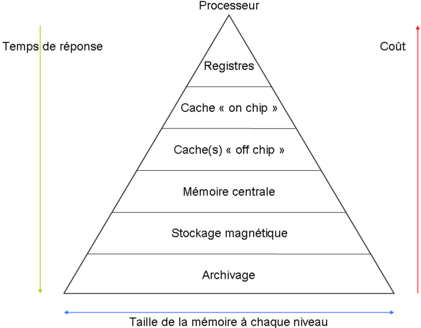
\includegraphics[scale=.6]{images/hierarchy.png}
	\end{figure}
	\begin{block}{Objectif}
		\begin{itemize}
			\item{Trouver un bon compromis entre vitesse et coût}
		\end{itemize}
	\end{block}
\end{frame}

%~ Ajouter définition de hit/miss
%~ Ajout d'une partie sur l'organisation interne d'un cache... (Set/ligne/bloc mémoire)

\begin{frame}{Associativité}
	\begin{block}{Comment localiser une donnée dans le cache ?}
		Il existe différentes fonctions de correspondance
		\begin{itemize}
			\item{Direct associative}
			\item{Fully associative}
			\item{k-ways associative}
		\end{itemize}
	\end{block}
	\begin{figure}[h!]
		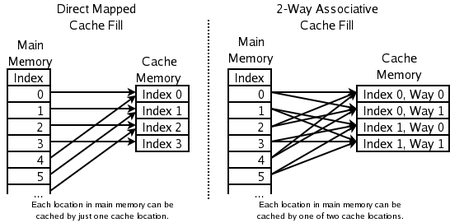
\includegraphics[scale=.4]{images/associative.png}
	\end{figure}
\end{frame}

\begin{frame}{Remplacement}
	\begin{block}{Comment ajouter une donnée dans cache plein ?}
		Il existe différentes politiques de remplacement
		\begin{itemize}
			\item{FIFO (Supprimer la plus ancienne)}
			\item{LFU (Supprimer la moins utilisée)}
			\item{LRU (Supprimer la plus anciennement utilisée)}
		\end{itemize}
	\end{block}
	Problème : Que deviennent les données évincées ?
\end{frame}

\begin{frame}{Hiérarchie de caches et problèmes de cohérence}
On utilise plusieurs niveaux de caches
%~  Schéma d'une hiérarchie de caches.
\begin{block}{Comment gérer les données entre différents niveaux?}
		\begin{itemize}
			\item{Caches inclusifs (Intel)}
			\item{Caches exclusifs (AMD)}
%~ Schéma d'illustration pour l'inclusivité ?
		\end{itemize}
	\end{block}
	\begin{block}{Comment gérer les données entre caches de même niveau?}
		Que faire lorsque deux caches doivent se partager une même donnée ?
	\end{block}
\end{frame}

\section{Gestion des politiques de coherence}

Les politiques de cohérence pré-implémentées sont MSI, MESI, MOESI, MESIF et MOSI. Elles sont nécessaires pour décrire l'état d'une ligne dans un cache et se représentent facilement par des automates dont les états sont ceux de la ligne, et les transitions sont des actions effectuées sur la ligne. Il est possible de rajouter d'autres politiques comme expliqué dans le tutoriel de la partie \ref{tuto_aut}, la section ci-dessous a pour vocation uniquement de préciser la paramétrisation des politiques déjà définies, sans évoquer la syntaxe à utiliser.

\subsection{Actions réalisées par une politique de cohérence}
\label{actions}

\paragraph{}
Une politique de cohérence est utilisée afin de garantir la cohérence des données dans tous les caches d'un même niveau : c'est-à-dire éviter qu'un cache ne possède une donnée qui n'est pas à jour car modifiée par un autre cache. L'objectif des constructeurs est donc de limiter les invalidations de lignes ou les messages de cohérence (voire l'envoi de la ligne) entre les caches, en cas de modification d'une ligne par un cache tiers. 

\paragraph{}
Dans le cas de \textsf{Cassis}, les politiques de cohérence s'occupent donc simplement de modifier le nouvel état de la ligne en cas d'action sur celle-ci. Les actions (qui sont donc les transitions des automates) peuvent être une lecture, une écriture ou une suppression, par le cache-même ou par un des caches du même niveau. Certaines statistiques dépendent aussi de ces actions. Ainsi les \verb!COHERENCE_EVINCTION!, \verb!COHERENCE_BROADCAST! et les \verb!WRITE_BACK! sont comptabilisées par les politiques de cohérence, respectivement dans le cas d'une invalidation de la ligne pour cause de modification dans un autre cache, pour l'envoi d'un message ou d'une donnée aux autres caches et enfin pour l'écriture de la donnée dans le cache parent. 

\subsection{Utilisation de SMC}

\paragraph{}
Afin de décrire facilement ces automates, l'utilsateur dispose d'un unique fichier à modifier qui contient toutes les desciptions de politiques. Celui-ci est rédigé grâce à un DSL -- Domain Specific Language -- nommé \textsf{SMC}, pour State Machine Compiler. Le fichier concerné est \verb!coherence.sm! situé au niveau des sources dans le dossier \verb!state-machine!. Il nécessite pour générer le code \texttt{C} associé d'une version standard de \texttt{Java}.

\paragraph{}
Ce DSL permet de définir plusieurs automates, dont les transitions sont les fonctions à appeler pour modifier leur état. \textsf{SMC} tel qu'utilisé dans le simulateur permet de réaliser plusieurs opérations : décrire les états de l'automate, décrire les transitions (entre états d'un même automate ou non), appliquer des conditions aux transitions, et enfin effectuer des actions spécifiques lors de l'appel d'une transition.

\paragraph{}
Certaines subtilités peuvent toutefois sembler complexe pour l'utilisateur : par exemple le nommage des fonctions possibles à l'intérieur du fichier de description. Les règles typographiques des transitions, et les possibilités d'action sont restreintes, voir pour cela la partie \ref{tuto_aut}.

\subsection{\'Ecriture d'une politique}

\paragraph{}
La première phase de l'écriture d'une politique est de pouvoir l'initialiser. En effet l'automate de départ n'est qu'un automate de départ vers les politiques : la première transition appelée correspond au choix de la politique, et va placer l'automate dans l'état I (\emph{invalid}) de la politique voulue. Il faut donc ajouter la transition dans l'automate de départ du fichier, automate nommé \texttt{Init} et ne comportant qu'un seul état mais autant de transitions que de politiques différentes.

\paragraph{}
Chaque politique doit donc contenir au moins l'état I ; et pour chaque état qu'elle définit elle peut ajouter des transitions, éventuellement conditionnelles. Les actions réalisées lors d'une transition doivent contenir à la fois les statistiques si nécessaires et à la fois la modification de l'état dans la structure contenant l'automate. En effet il n'a pas été possible de récupérer l'état courant de l'automate nécessaire à certaines fonctions. Cet état doit donc être sauvegardé dans la structure d'une ligne, en plus de la structure même de l'automate. Il s'agit d'une duplication d'information nécessaire au fonctionnement général du simulateur, et dû à des problèmes d'interfaçage entre le \texttt{C} et \textsf{SMC}.

\paragraph{}
\`A la fin de chaque description de politique se trouve un certain de nombre de transitions par défaut. Si elles sont appelées sur un état ne les définissant pas, elles bouclent dessus. Cela sert à factoriser les transitions n'effectuant aucune action sur un état.

\subsection{\'Eléments paramétrisables}

\paragraph{}
Les éléments dits paramétrisables de ce fichier, sont ceux qui ne nécessitent pas d'intervention dans d'autres fichiers du code source. Il n'est ainsi pas possible de rajouter de nouveau type de transition ou de nouvel automate, car ceux-ci ne seraient pas appelées par le programme principal. Sont donc modifiables : \\
\begin{itemize}
\item{les noms des états et des automates, il est aussi possible d'enlever ou d'ajouter d'autres états,}
\item{les actions des transitions, i.e. la modification de l'état tel que visible par le simulateur et l'incrémentation d'une statistique déjà existante,}
\item{les transition conditionnelles (en rajouter ou supprimer mais uniquement en utilisant les fonctions de tests préexistantes),}
\item{les transitions par défaut et actions associées (en rajouter ou supprimer).}
\end{itemize}

\paragraph{}
Deux fonctions sont disponibles pour les tests des transitions conditionnelles, il s'agit pour l'une de savoir si une ligne est marquée comme \emph{dirty} ou non, et pour l'autre de savoir si une ligne est présente ailleurs dans le niveau, avec possibilité de chercher une ligne dans un état spécifique. Attention, si l'état en paramètre est I, alors ce sont toutes les lignes valides qui sont recherchées. Il n'est donc pas possible de savoir si une ligne est dans l'état I ailleurs dans le niveau.




\begin{frame}[fragile]
  \frametitle{Données d'entrée de \emph{Cassis}}
  
%  \begin{figure}[h!]
%    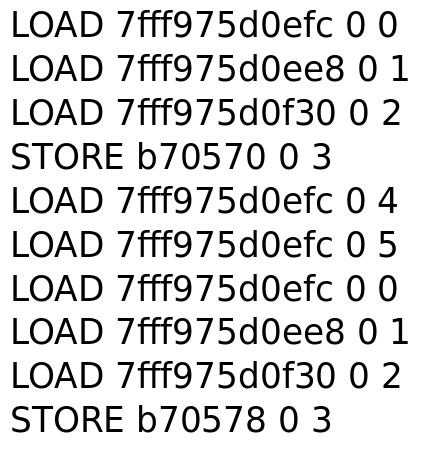
\includegraphics[width=.4\textwidth]{images/traces.png}
%  \end{figure}
  
  \begin{itemize}
    \item Fichier de description d'architecture
    \item Trace d'exécution
  \end{itemize}
  
\begin{verbatim}
LOAD 7fff975d0efc 0 0
LOAD 7fff975d0ee8 0 1
LOAD 7fff975d0f30 0 2
STORE b70570 0 3
LOAD 7fff975d0efc 0 4
LOAD 7fff975d0efc 0 5
LOAD 7fff975d0efc 0 0
LOAD 7fff975d0ee8 0 1
LOAD 7fff975d0f30 0 2
STORE b70578 0 3
...
\end{verbatim}

\end{frame}

\begin{frame}
  \frametitle{Lecture d'une ligne par le simulateur}
  
  \begin{figure}[h!]
    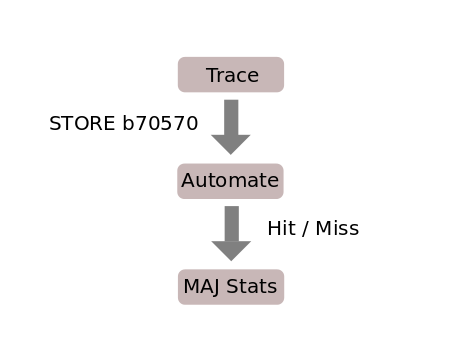
\includegraphics[width=.8\textwidth]{images/cassis_deroulement.png}
  \end{figure}
  
\end{frame}


\section{Paramétrisation de l'architecture}

L'architecture à simuler peut être générée à partir de l'architecture réelle de l'utilisateur au moyen d'un fichier XML créé par le logiciel \emph{HWLOC}. Cependant l'utilisateur peut utiliser un fichier de paramétrisation spécifique à notre simulateur qui lui permet d'accéder à l'intégralité des paramètres d'architecture pris en compte.

\subsection{Entrée XML HWLOC}

\emph{HWLOC} est un logiciel libre sous liscence BSD-2. Il permet de générer un fichier XML qui décrit l'architecture de la machine utilisée (commande \verb?lstopo --of xml?). Il décrit notamment la structure arborescente des caches, et donne des informations essentielles pour chaque cache, comme sa taille, la taille de ses lignes et son associativité. 

\paragraph{}
Si l'utilisateur choisit un tel fichier en entrée comme décrivant son architecture, ce dernier sera parsé en un fichier de configuration de l'architecture personnalisé, comme décrit dans la section \ref{config}. Les paramètres non fournis par le fichier généré par \emph{HWLOC} prendront des valeurs par défaut, proches de celles des architectures \emph{intel} moderne. Notons que notre simulateur ne prend pas en compte les caches de niveau 1 dédiés aux instructions (L1i), qui sont décrits par \emph{HWLOC} mais ne seront pas présent dans le fichier personnalié.

\subsection{Fichier de configuration personnalisé}
\label{config}
Le fichier de configuration de l'architecture dédié à notre simulateur comprend tous les paramètres d'achitecture utilisables. Une fois généré à partir d'un fichier \emph{HWLOC}, il est possible de l'utiliser directement en entrée du simulateur, après avoir été modifié à la convenance de l'utilisateur.

\paragraph{}
Il s'agit d'un fichier XML qui contient 3 balises :
\begin{itemize}
  \item \textbf{Architecture} : donne le nom de l'architecture et du modèle de microprocesseur utilisé, ainsi que le nombre de niveaux de cache.
  \item \textbf{Level} : décrit un niveau de cache. Pour chaque profondeur, le protocole de cohérence, le type d'inclusivité, la présence ou non de \textit{snooping} et d'un \textit{directory manager}.
  \item \textbf{Cache} : décrit l'arborescence des caches. Pour chaque cache, sa profondeur, sa taille, la taille de ses lignes, son associtivité et son protocole de remplacement.
\end{itemize}

\subsubsection{Paramètres de la balise Architecture}

\begin{itemize}
  \item \textbf{name} : nom de l'architecture (ex : \textit{x86\_64})
  \item \textbf{CPU\_name} : modèle du microprocesseur
  \item \textbf{number\_levels} : nombre de niveaux de cache
\end{itemize}

\subsubsection{Paramètres de la balise Level}

\begin{itemize}
  \item \textbf{depth} : la profondeur du niveau. La valeur doit être cohérente avec le nombre de niveaux de l'architecture.
  \item \textbf{coherence\_protocol} : \verb?MESI? ou \verb?MSI?
  \item \textbf{type} : \verb?inclusive?, \verb?exclusive?, \verb?niio? (Non Inclusive, Inclusive Oriented) ou \verb?nieo? (Non Inclusive, Exclusive Oriented)
  \item \textbf{snooping} : \verb?true? ou \verb?false?
  \item \textbf{directory\_manager} : \verb?true? ou \verb?false?
\end{itemize}

\subsubsection{Paramètres de la balise Cache}
Ces balises doivent former l'arborescence des caches.

\begin{itemize}
  \item \textbf{depth} : la profondeur du cache.
  \item \textbf{cache\_size} : taille du cache (en octets)
  \item \textbf{cache\_linesize} : taille d'une ligne de cache (en octets)
  \item \textbf{cache\_associativity} : associativité du cache
  \item \textbf{remplacement\_protocol} : \verb?FIFO?, \verb?LRU? ou \verb?LFU?
\end{itemize}

\subsubsection{Exemple de fichier}

%TODO : mettre un exemple de fichier à jour

\subsection{\'Etapes de validation}
\begin{frame}
  \begin{block}{Pr\'esentation}
    \begin{itemize}
      \item Tests unitaires
      \item Validation durant le programme
      \item Comparaison avec des outils existants
      \item Benchmarks
    \end{itemize}
  \end{block}
  \begin{block}{Premiers outils de v\'erification}
    \begin{itemize}
      \item Validation des politiques basiques
      \item Validation du comportement inclusif
      \item Utilisation de \textsf{PAPI}
    \end{itemize}
  \end{block}
\end{frame}

\begin{frame}{Benchmarks basiques}
\begin{figure}[H]
   \begin{minipage}[l]{.46\textwidth}
     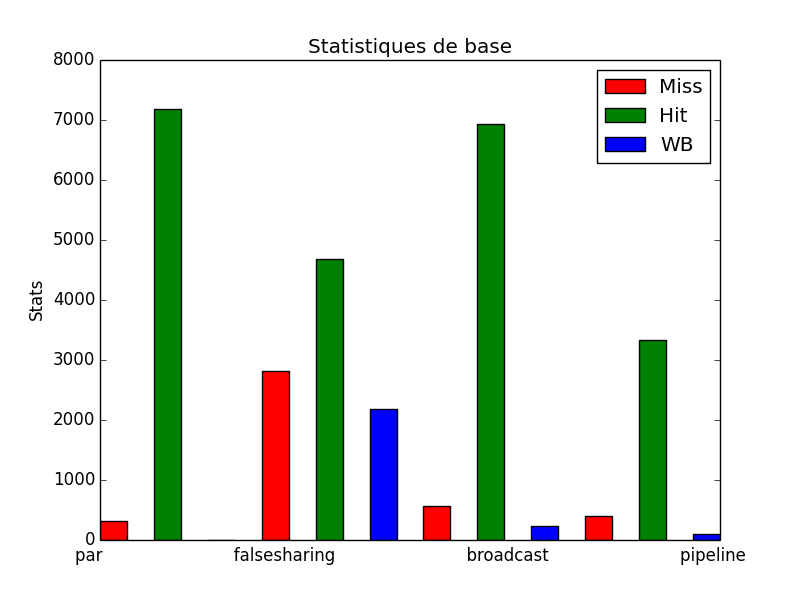
\includegraphics[scale=0.22]{images/stats_L1.png}
   \end{minipage} \hfill
   \begin{minipage}[r]{.46\textwidth}
     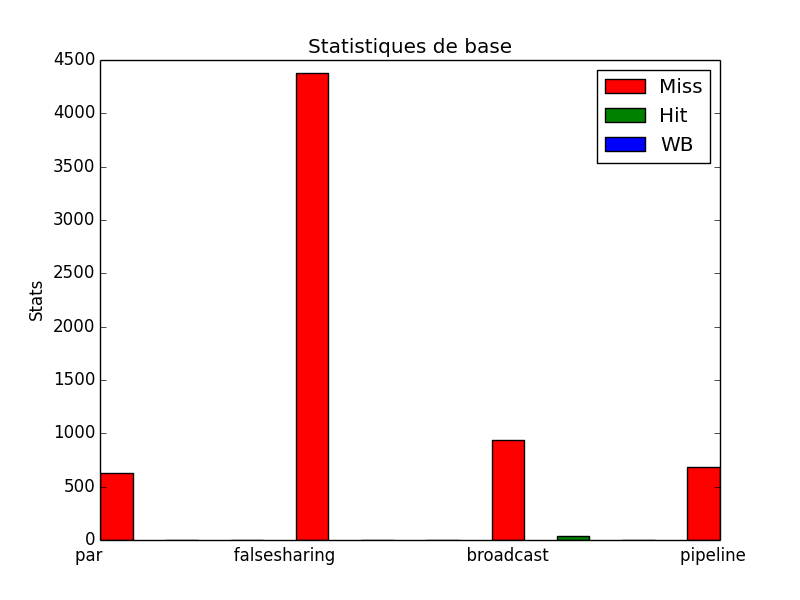
\includegraphics[scale=0.22]{images/stats_L2.png}
   \end{minipage}
\end{figure}

\begin{figure}[t!]
  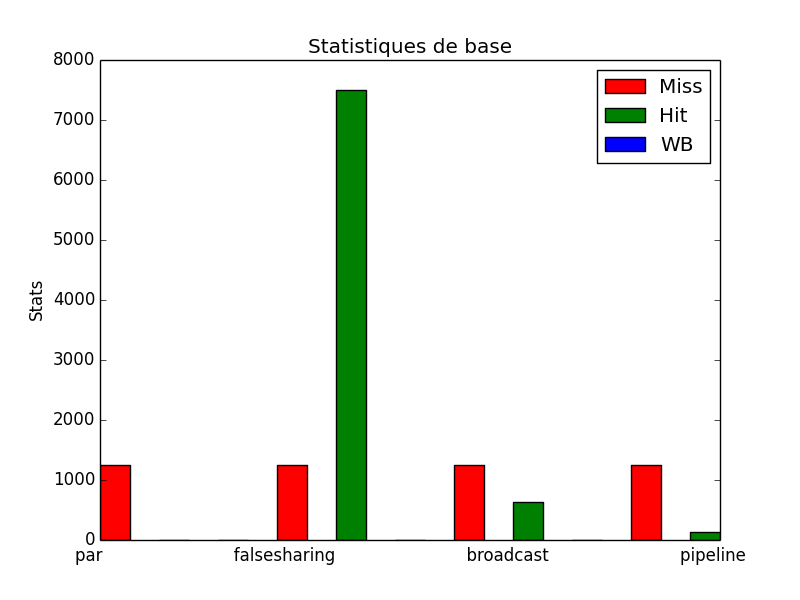
\includegraphics[scale=0.22]{images/stats_L3.png}
\end{figure}
\end{frame}

\begin{frame}{Benchmarks avanc\'es}
\begin{figure}[H]
   \begin{minipage}[l]{.46\textwidth}
     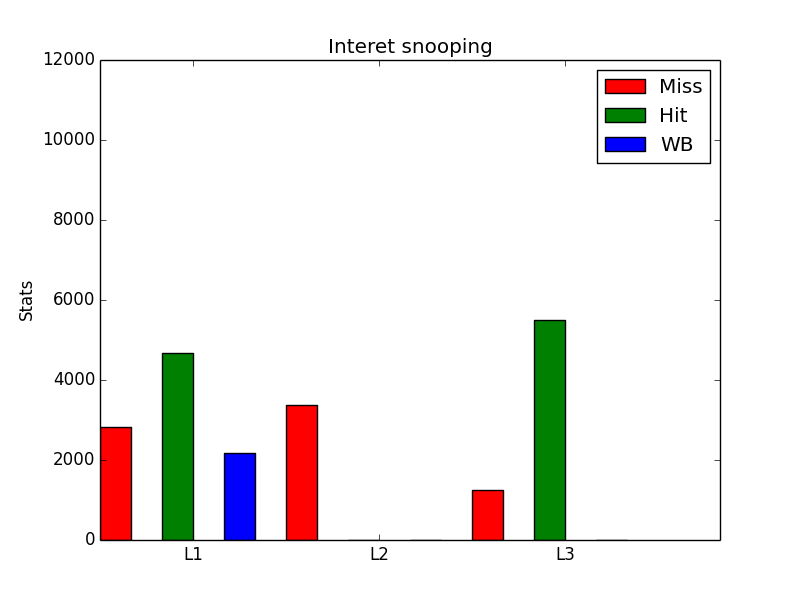
\includegraphics[scale=0.22]{images/stats_falsesharing_snooping.png}
   \end{minipage} \hfill
   \begin{minipage}[r]{.46\textwidth}
     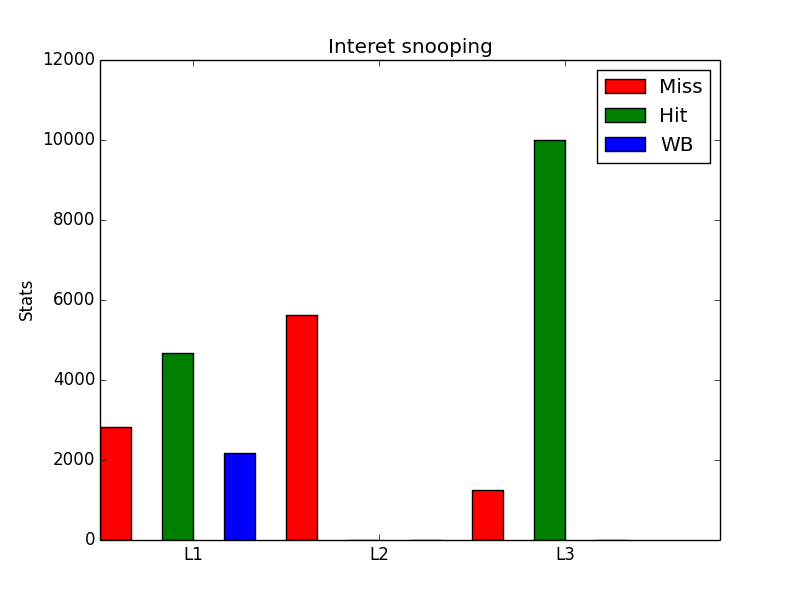
\includegraphics[scale=0.22]{images/stats_falsesharing_no_snooping.png}
   \end{minipage}
\end{figure}
  \begin{block}{Autres benchmarks}
    \begin{itemize}
      \item \emph{Directory manager}
      \item Politiques de coh\'erence MSI vs MESI
      \item Scalabilit\'e
    \end{itemize}
  \end{block}
\end{frame}

\subsection{Limites \`a  propos de la simulation des caches}
\begin{frame}
  \begin{block}{Probl\`emes li\'es aux architectures multi-c{\oe}ur}
    \begin{itemize}
      \item \textsf{prefetching}
      \item synchronisations
      \item changements de contextes 
    \end{itemize}
  \end{block}
  \begin{block}{Limites de \textsf{Cassis}}
    \begin{itemize}
      \item bande passante non mod\'elis\'ee
      \item \textsf{Directory manager} basiquement mod\'elis\'es
      \item statistiques non calibr\'ees avec des benchmarks classiques
      \item utilisation de m\'etriques non usuelles
    \end{itemize}
  \end{block}
\end{frame}


\section*{Conclusion}
\begin{frame}
  \begin{block}{Objectifs atteints}
    \begin{itemize}
      \item Cahier des charges respect\'e
      \item Param\'etrisation compl\`ete
    \end{itemize}
  \end{block}

  \begin{block}{\'Evolution possible}
    \begin{itemize}
      \item Complage avec un simulateur \textsf{on-line}?
      \item Utilisation de benchmarks pour calibrer les r\'esultats?
    \end{itemize}
  \end{block}
\end{frame}


\end{document}
